%
\section{Introduction}%
%
\begin{frame}[t]%
\frametitle{Introduction}%
\bigskip%
\begin{itemize}%
\item Benchmarking of optimization algorithms is \only<2->{incredibly }important\uncover<3->{, but cumbersome}%
\item<4-> Tool support is needed\uncover<5->{, examples are BBOB's COCO\scitep{HAFR2012RPBBOBES}, \tspSuite\scitep{WCTLTCMY2014BOAAOSFFTTSP}, UBCSAT\scitep{TH2004UAIAEEFSAFSAMS}, or AOAB\scitep{WNT2010AOABAOAB}\uncover<6->{ -- which are all \inQuotes{field-specific}}}
\item<7-> Can we design a general tool for evaluating results from experiments with optimization algorithms?%
\\~\bigskip~\\\bigskip~\\\bigskip~\\\medskip%
\item<8-> {\textbf{\Large{\alert{\optimizationBenchmarking\ is an attempt to do just that.}}}}%
\end{itemize}%
\locateFramedGraphic{8}{width=0.4\paperwidth}{graphics/logo/logo}{0.3}{0.2}%
\end{frame}%
%
\begin{frame}[t]%
\frametitle{Experimental Procedure}%
\begin{itemize}%
\item In optimization or Machine Learning, the following experimental procedure is often used\uncover<2->{%
\begin{enumerate}%
\item Select a \only<3->{\alert<3>{set of }}benchmark instance\only<3->{\alert<3>{s}}\only<3-7>{:%
\begin{itemize}%
\item multiple instances%
\item<4-> which cover some different problem features%
\item<5-> should be well-known to make results comparable%
\only<-6>{%
\item<6-> e.g., TSPLib\scitep{R1991ATSPL,R1995T9,DACO1995TSPLIB} for the TSP has instances with different numbers of cities and geometries%
}%
\only<-7>{%
\item<7-> e.g., BBOB\scitep{HAFR2012RPBBOBES,NAFR2010RPBBOB2ES,HAFR2009RPBBOB2ES,FHRA2013RPBBOB2POTNF} offers different benchmark functions for numerical optimization problems%
}%
\end{itemize}%
}%
\item<8-> Do experiment\only<12->{\alert<12-13>{s}}\only<9-13>{:%
\begin{itemize}%
\item conduct several independent runs of algorithm for each benchmark instance%
\item<10-> collect algorithm progress information, e.g., as \emph{\inQuotes{runtime bestObjectiveValue}} tuples%
\item<11-> one log file per run, each log file has several such tuples%
\item<12-> repeat for different algorithm parameter settings (e.g., different population sizes of an EA)%
\item<13-> repeat with other algorithms for comparison purposes%
\end{itemize}%
}%
\item<14-> Evaluate the gathered data\only<15->{:\alert<22>{%
\begin{itemize}%
\item draw diagrams of progress of solution quality over time%
\item<16-> draw diagrams of advanced statistical parameters such as ECDF\scitep{HAFR2012RPBBOBES,HS1998ELVAPAR,TH2004UAIAEEFSAFSAMS,WCTLTCMY2014BOAAOSFFTTSP}\only<17->{ and ERT\scitep{HAFR2012RPBBOBES,WCTLTCMY2014BOAAOSFFTTSP}} (over time)%
\item<18-> use statistical tests to compare results (at different points during the runs)%
\item<19-> analyze the impact of benchmark features and algorithm parameters on the above%
\end{itemize}%
}}%
%
\item<20-> Draw conclusions about algorithm performance and parameter settings%
\item<21-> But this is all \emph{very} cumbersome, involves much work and much data\dots%
\end{enumerate}%
}%
\item<22-> \alert{The \optimizationBenchmarking\ framework can automatize much of the evaluation procedure}%
\end{itemize}%
%
\locateWithCaption{6}{%
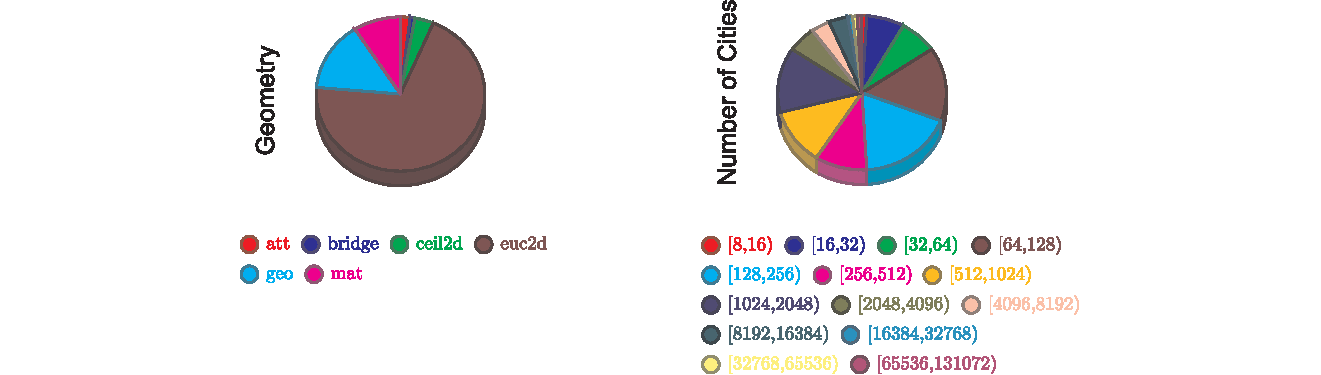
\includegraphics[width=0.925\paperwidth]{graphics/tspLib_features/tspLib_features_symmetric}%
}{%
The relative amounts of the instances of the 110 symmetric instances of TSPLib according to their features (the 10 asymmetric instances are not plotted).%
}{0.0375}{0.51}{0.925}%
%
\locateWithCaption{7}{%
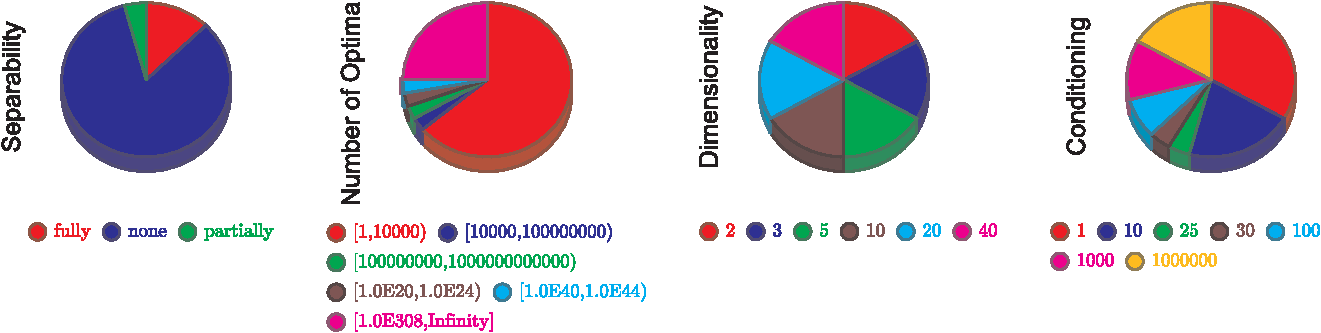
\includegraphics[width=0.925\paperwidth]{graphics/bbob_features/bbob_features}%
}{%
The relative amounts of BBOB benchmark functions according to their features.%
}{0.0375}{0.51}{0.925}%
%
\locateWithCaption{10}{%
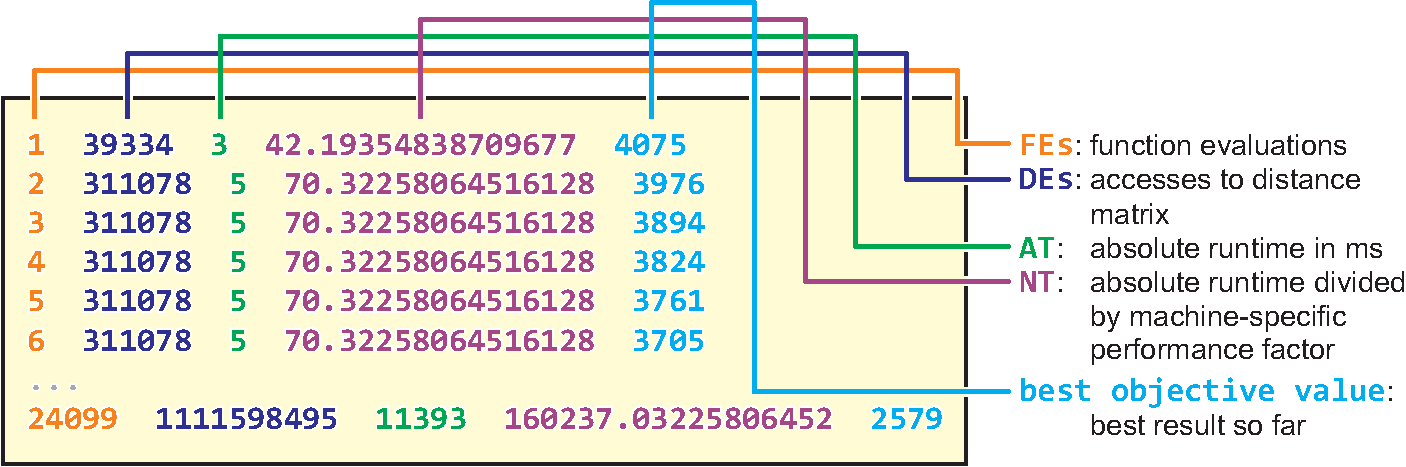
\includegraphics[width=0.8\paperwidth]{graphics/tspSuite_logfile_example/tspSuite_logfile_example}%
}{%
Example for data collected in a log file by TSP~Suite\scitep{WCTLTCMY2014BOAAOSFFTTSP,JWLCA2014CAHBABAWECMLSATHOTT}.%
}{0.0375}{0.53}{0.925}%
%
\locateWithCaption{15-17}{
\strut%
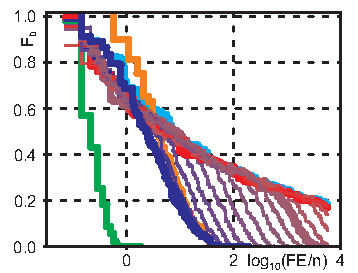
\includegraphics[width=0.28\paperwidth]{graphics/performance/progress_example/progress_example}%
\uncover<16->{%
\strut\hfill\strut%
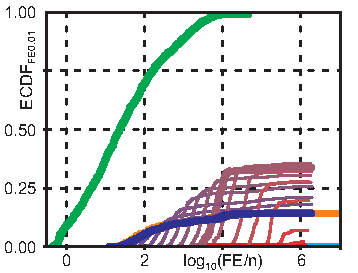
\includegraphics[width=0.28\paperwidth]{graphics/performance/ecdf_example/ecdf_example}%
\uncover<17->{%
\strut\hfill\strut%
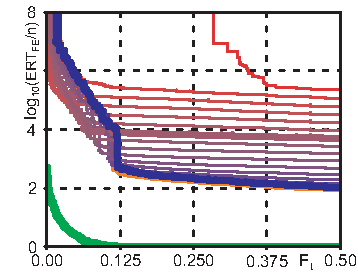
\includegraphics[width=0.28\paperwidth]{graphics/performance/ert_example/ert_example}%
}}\strut%
}{%
Examples for progress\only<16>{ and ERT}\only<17->{, ERT, and ECDF} diagrams for different algorithms (signified by different colors) over different sub-sets of the TSPLib data.%
}{0.0375}{0.525}{0.925}%
%
\end{frame}%
